%%
%% Desenvolvimento.tex
%% Projeto Oficinas de Integração 3
%% Created by Leonardo Winter Pereira and Lucas Zimmermann Cordeiro on 10.03.2016
%% Copyright (C). All rights reserved
%%

\chapter{Desenvolvimento}
\label{chap:desenvolvimento}



    \section{Hardware}



    \section{Estação Base Principal}



        \subsection{Interface}



        \subsection{Lógica}



    \section{Estação Base Secundária}



        \subsection{Interface}



        \subsection{Lógica}



    \section{Comunicação entre Hardware e Software}

        Nesta seção discutiremos como foi realizada a comunicação entre o Hardware e o Software do Dalle Pad.

    \section{Projeto Mecânico}

        O desenvolvimento do projeto mecânico é uma das etapas mais importantes de qualquer projeto, e o \textbf{Dalle Pad} não é exceção.
        
        Um bom projeto mecânico deve considerar diversos quesitos, tais como resistência, momento, peso tamanho (tanto interno como externo) do produto. Este projeto procura unir todos os quesitos acima citados, além de manter os custos de produção o mais baixo possível. Para que isso fosse possível, a equipe responsável decidiu projetar todos os componentes em uma ferramenta específica, podendo assim ser consideradas todas as variáveis para desenvolver um projeto de sucesso.
        
        Esta seção, inicialmente, apresenta ao leitor os componentes, adquiridos já em sua forma final, utilizados no decorrer do desenvolvimento do invólucro. Em seguida, serão apresentados os componentes projetados e produzidos especialmente para este projeto. Por último, apresenta-se o produto em sua forma final.
        
        \subsection{Componentes terceirizados}
        
            No decorrer deste projeto, diversos componentes puderam ser adquiridos prontos, o que auxiliou na redução de custos do mesmo, além de diminuir o trabalho de toda a equipe.

            Os seguintes componentes foram utilizados:

            \begin{itemize}
                \item \sigla{PCI}{Placa de Circuito Impresso} MIDI:

                    \begin{figure}[H]
                        \centering
                        \begin{subfigure}{.5\textwidth}
                          \centering
                          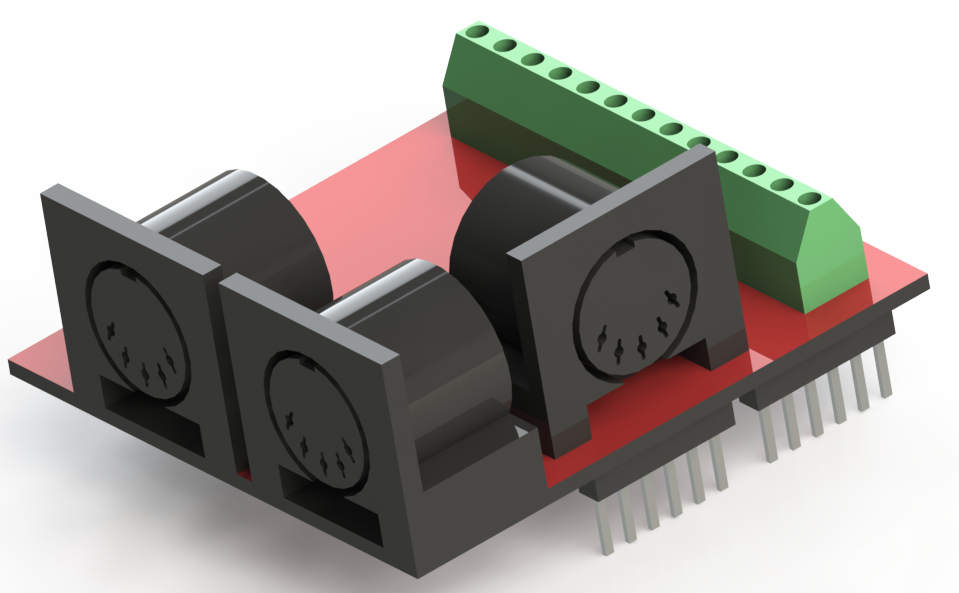
\includegraphics[scale=0.2]{Imagens/SW_Images/midi_shield1.png}
                          \caption{Vista 1}
                          \label{fig:MIDI_SHIELD_1}
                        \end{subfigure}%
                        \begin{subfigure}{.5\textwidth}
                          \centering
                          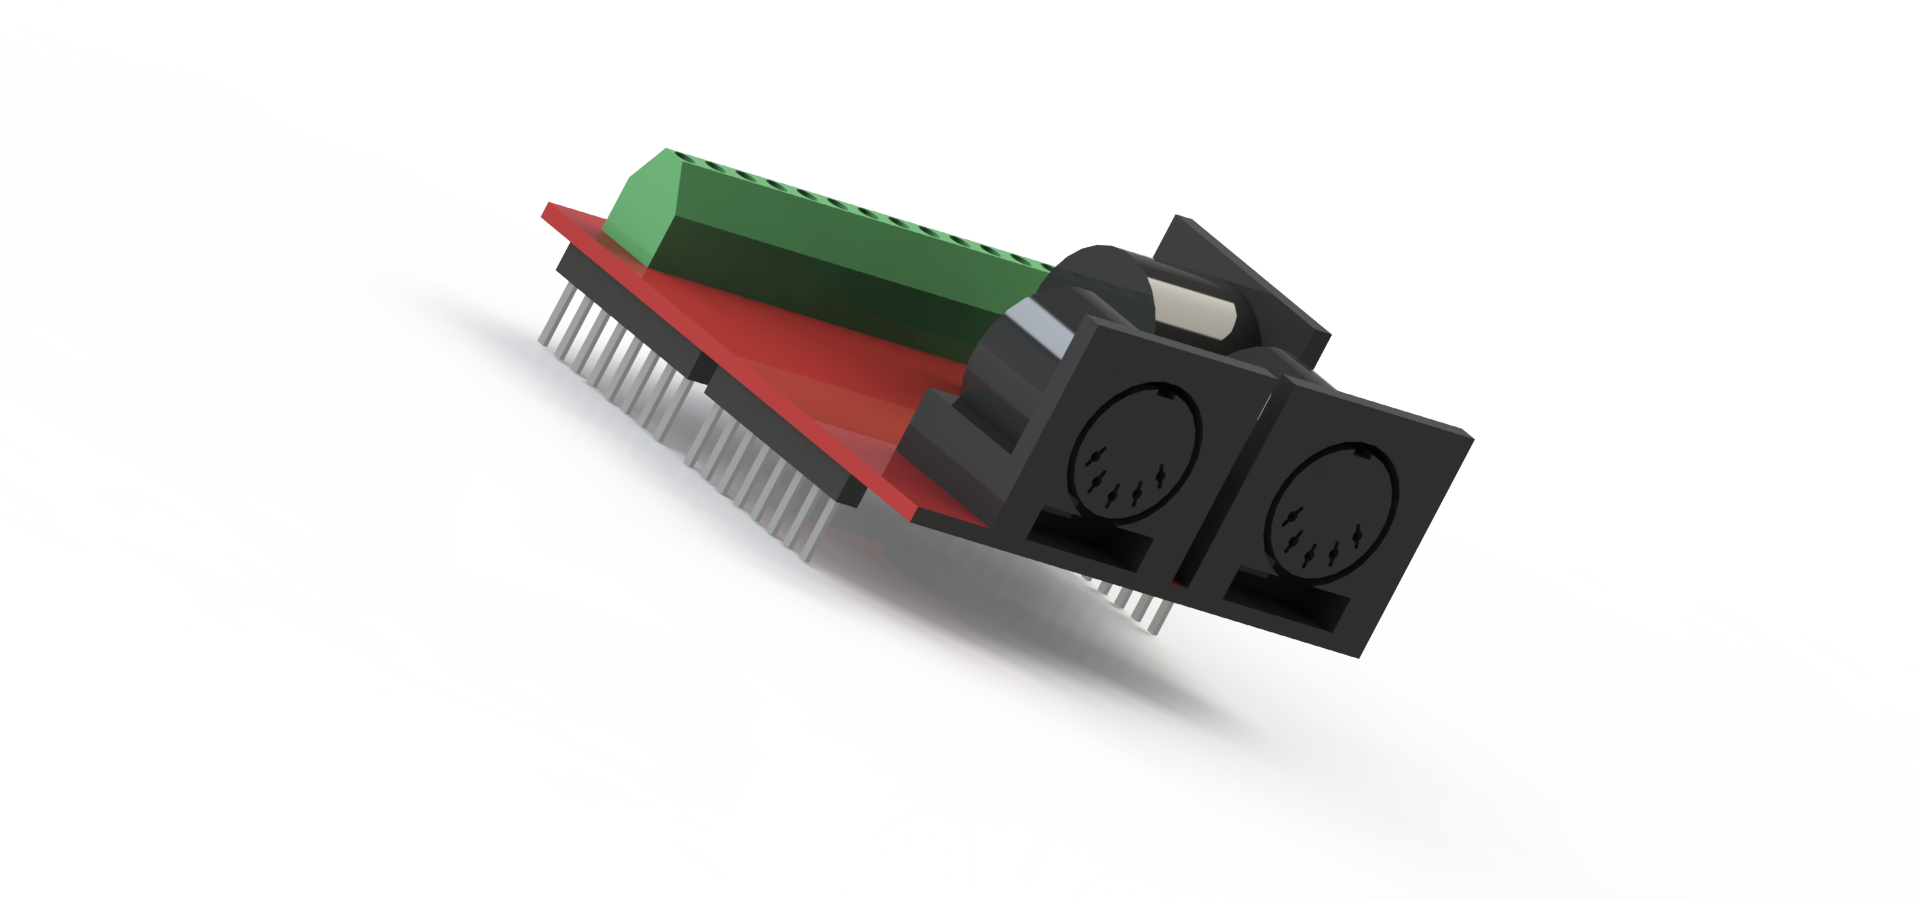
\includegraphics[scale=0.2]{Imagens/SW_Images/midi_shield2.png}
                          \caption{Vista 2}
                          \label{fig:MIDI_SHIELD_2}
                        \end{subfigure}
                        \caption{PCI MIDI}
                        \label{fig:MIDI_SHIELD}
                    \end{figure}

                \item Potenciômetro Linear:

                    \begin{figure}[H]
                        \centering
                        \begin{subfigure}{.5\textwidth}
                          \centering
                          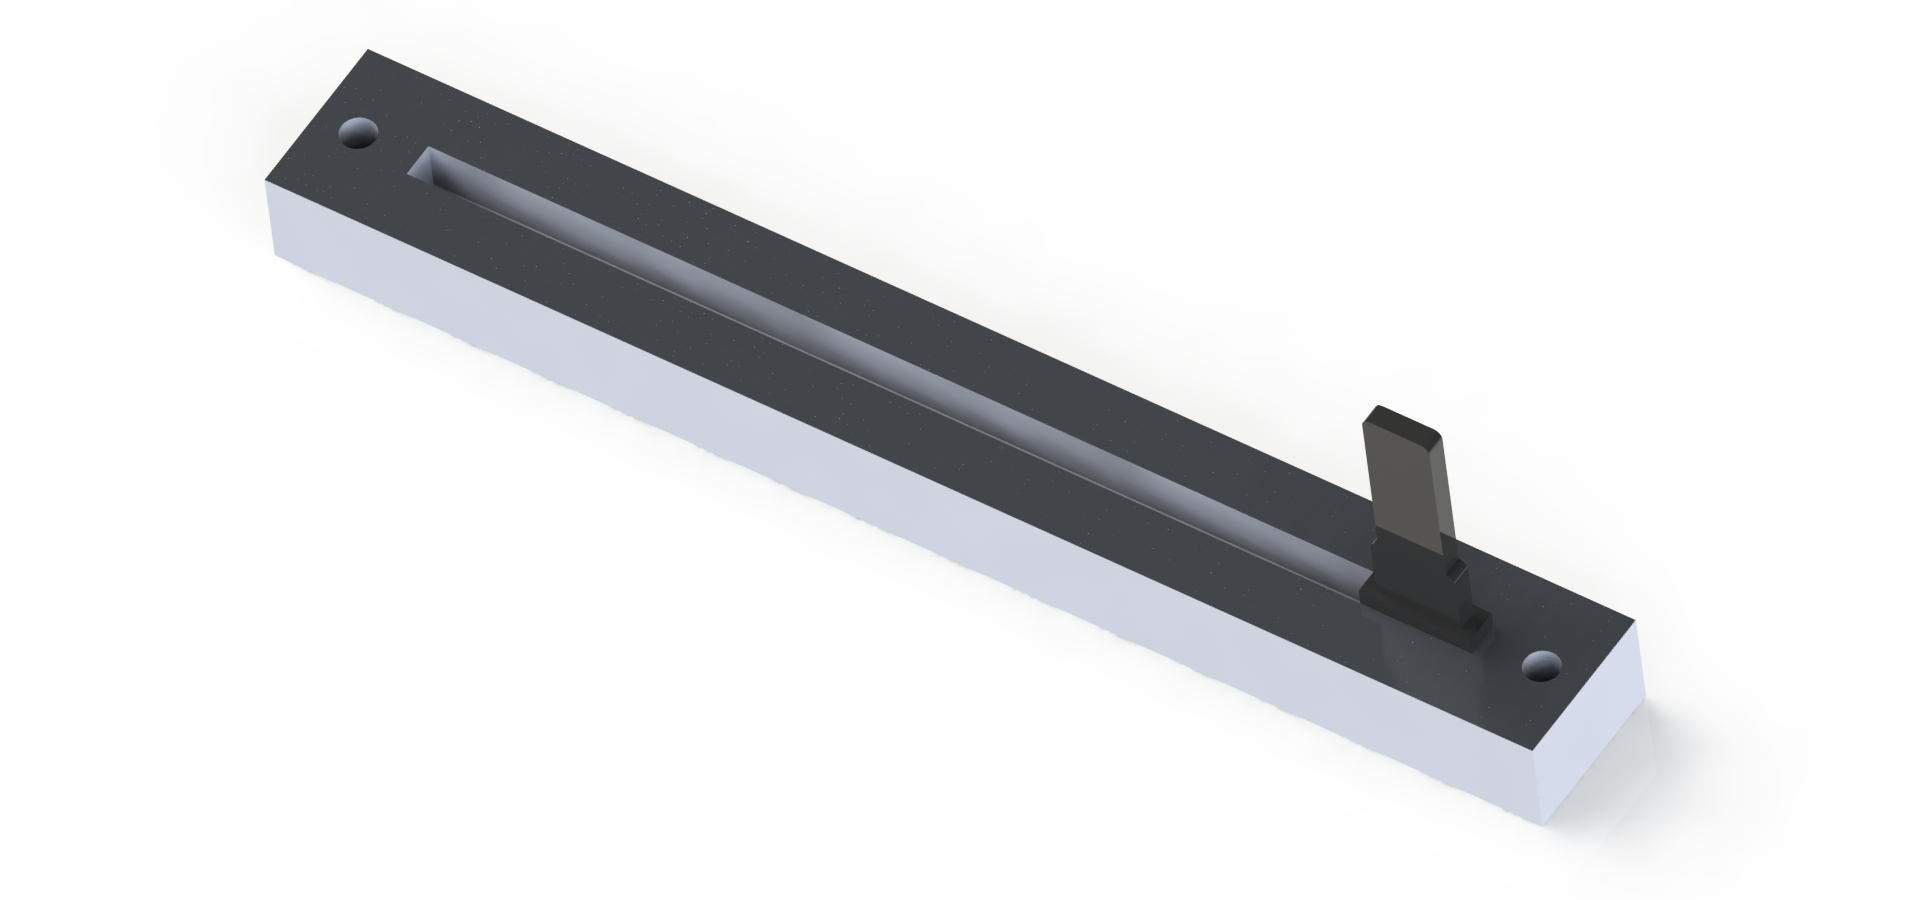
\includegraphics[scale=0.13]{Imagens/SW_Images/sliding_pot_b10k_capa.png}
                          \caption{Sem protetor}
                          \label{fig:Linear_Potentiometer_without_protector}
                        \end{subfigure}%
                        \begin{subfigure}{.5\textwidth}
                          \centering
                          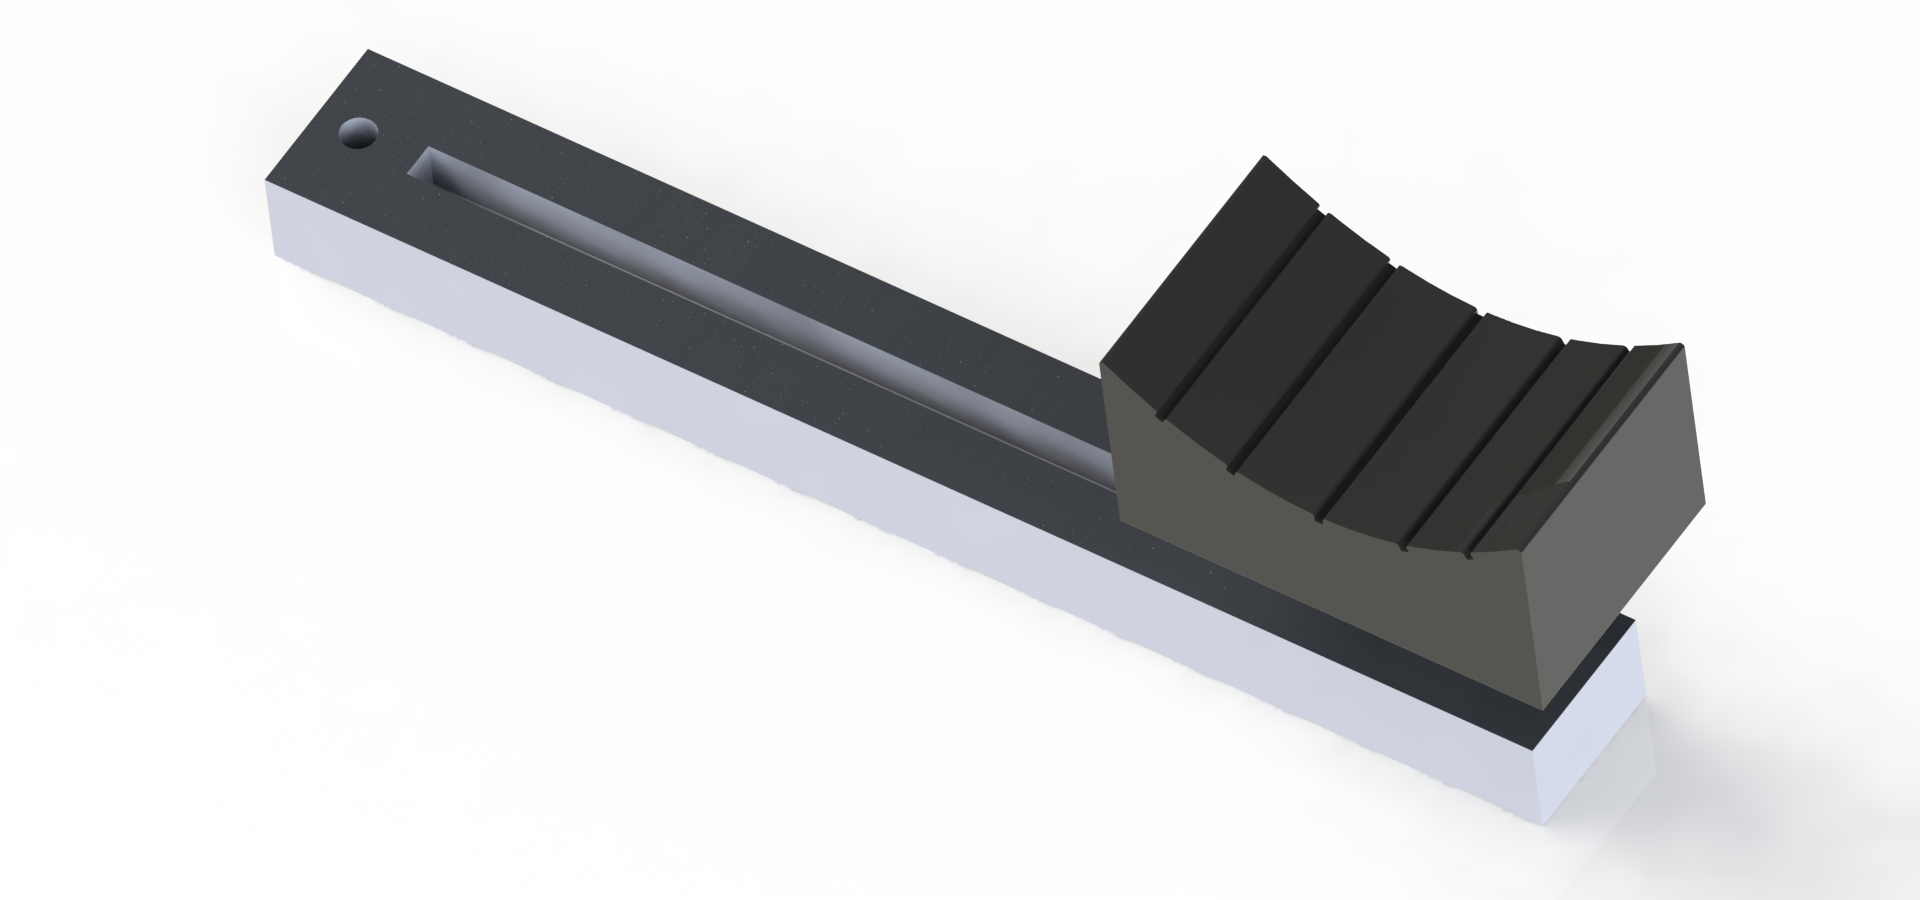
\includegraphics[scale=0.13]{Imagens/SW_Images/sliding_pot_b10k_montado.png}
                          \caption{Com protetor}
                          \label{fig:Linear_Potentiometer_with_protector}
                        \end{subfigure}
                        \caption{Potenciômetro linear B10K}
                        \label{fig:Linear_Potentiometer}
                    \end{figure}

                \item Potenciômetro Rotatório:

                    \begin{figure}[H]
                        \centering
                        \begin{subfigure}{.5\textwidth}
                          \centering
                          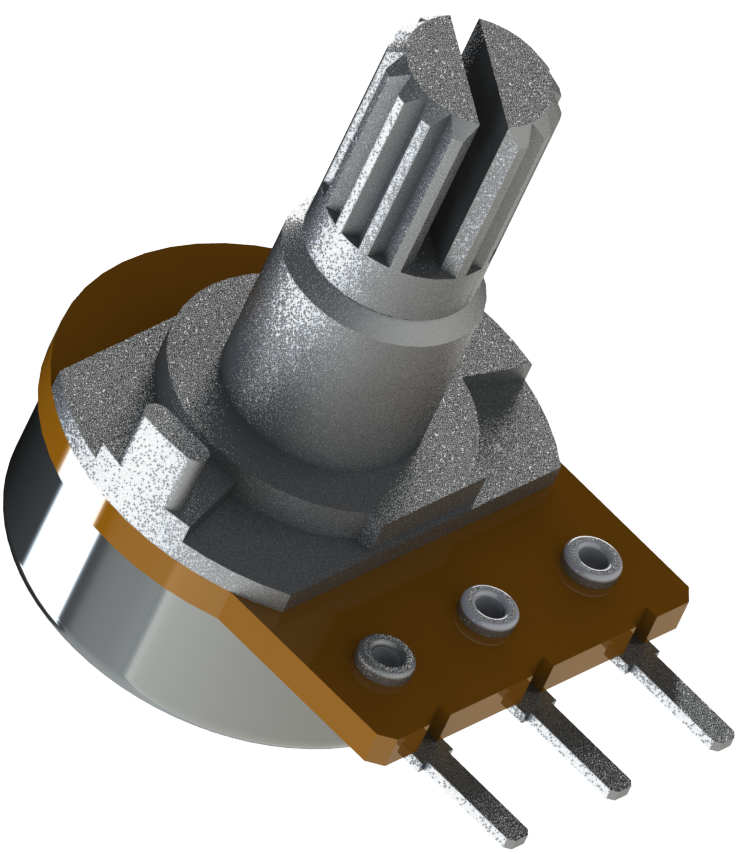
\includegraphics[scale=0.2]{Imagens/SW_Images/potentiometer-10k-2.png}
                          \caption{Sem protetor}
                          \label{fig:Rotary_Potentiometer_without_protector}
                        \end{subfigure}%
                        \begin{subfigure}{.5\textwidth}
                          \centering
                          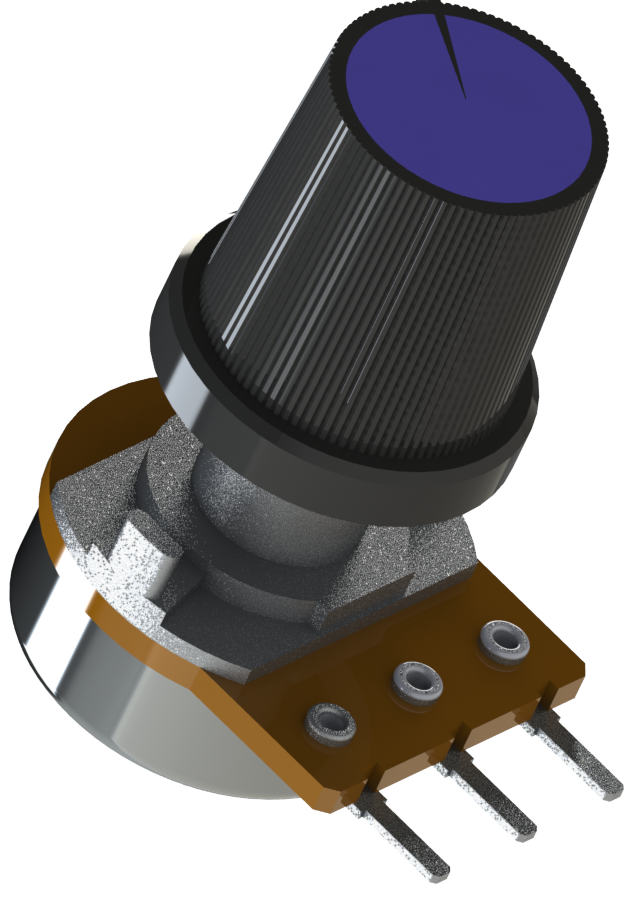
\includegraphics[scale=0.2]{Imagens/SW_Images/potentiometer-10k-1.png}
                          \caption{Com protetor}
                          \label{fig:Rotary_Potentiometer_with_protector}
                        \end{subfigure}
                        \caption{Potenciômetro rotatório B10K}
                        \label{fig:Rotary_Potentiometer}
                    \end{figure}

                \item Botão estilo ARCADE:

                    \begin{figure}[H]
                    	\centering
                    	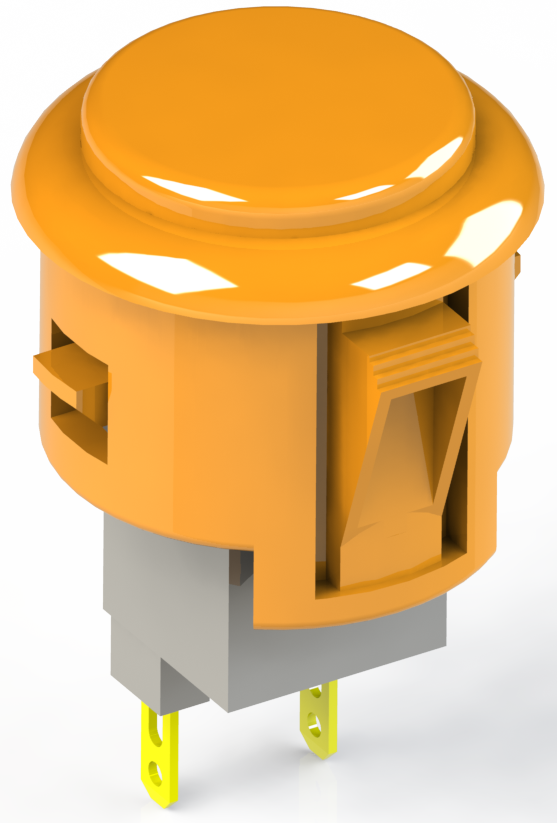
\includegraphics[scale=0.2]{Imagens/SW_Images/arcade_button.png}
                    	\caption[Botão estilo ARCADE]{Botão estilo ARCADE}
                    	\label{fig:Arcade_button}
                    \end{figure}
            \end{itemize}
            
        \subsection{Componentes projetados}
        
            Devido ao fato de todos os componentes mecânicos, estes necessários para o funcionamento do projeto, terem sido adquiridos prontos, foi necessário apenas projetar o invólucro do produto. Entretanto, o desenvolvimento deste não foi simples, devido ao fato de que o desejado era um produto compacto.
            
            A primeira etapa foi desenvolver a parte superior (veja as figuras ~\ref{fig:top_dalle_pad_01} e ~\ref{fig:top_dalle_pad_02}) e inferior (veja a figura ~\ref{fig:bottom_dalle_pad}) do invólucro. O mais importante foi planejar uma maneira eficiente de encaixar uma parte na outra, sem ocupar muito espaço interior.
            
            Também foi planejado encaixes para o Arduino e para a PCI MIDI, para que estes fiquem firmes e em posições onde o \textbf{Dalle Pad} apresentará maior resistência contra momento e pressão.
            
            \begin{figure}[H]
            	\centering
            	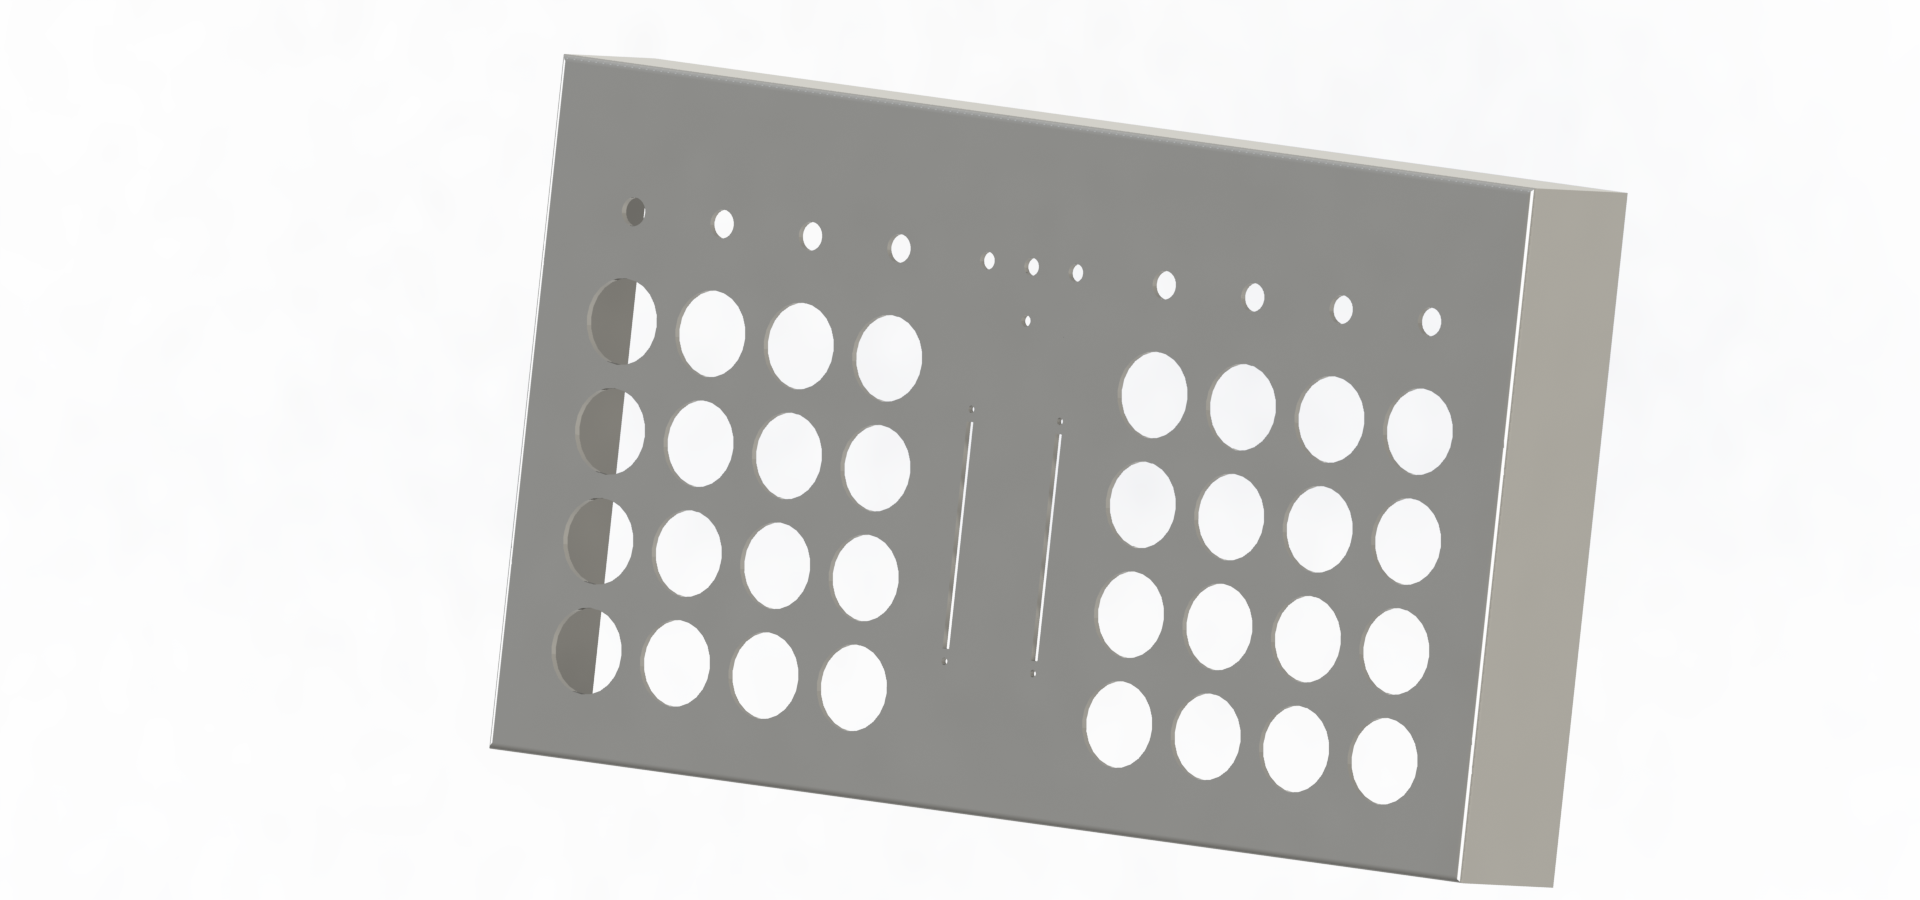
\includegraphics[scale=0.3]{Imagens/SW_Images/dalle_pad_capa_superior1.png}
            	\caption[Parte superior do invólucro - vista isométrica]{Parte superior do invólucro - vista isométrica}
            	\label{fig:top_dalle_pad_01}
            \end{figure}
            
            \begin{figure}[H]
            	\centering
            	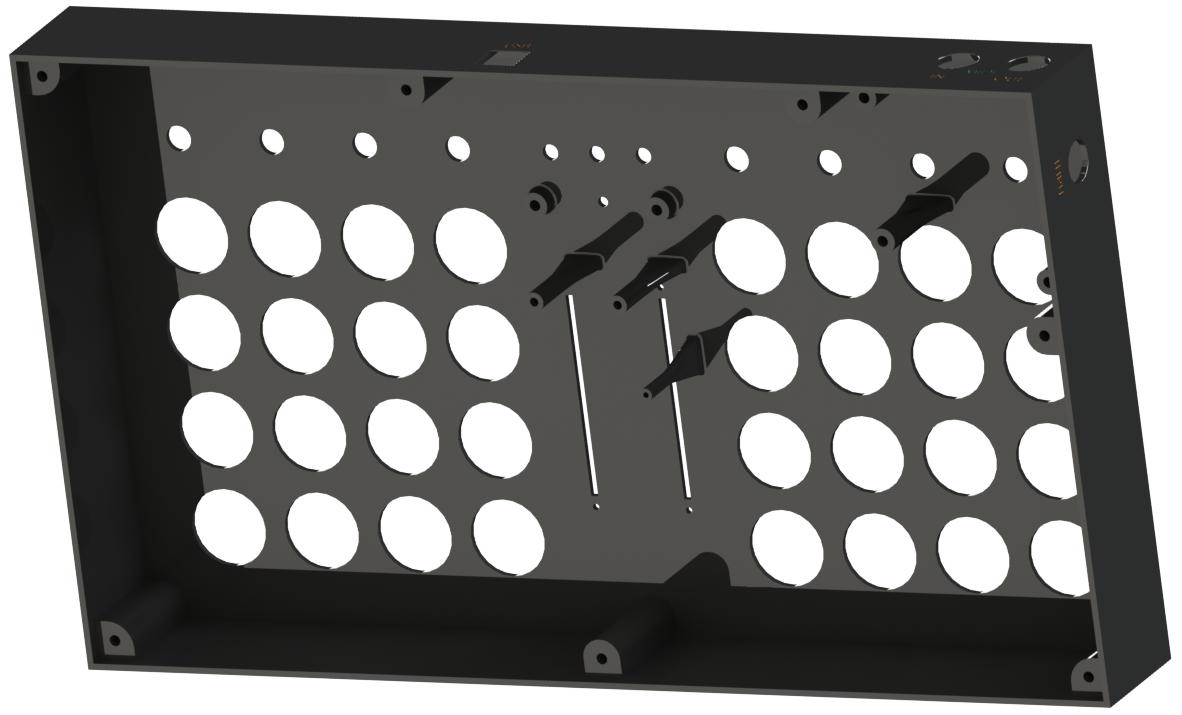
\includegraphics[scale=0.3]{Imagens/SW_Images/dalle_pad_capa_superior2.png}
            	\caption[Parte superior do invólucro - vista traseira]{Parte superior do invólucro - vista traseira}
            	\label{fig:top_dalle_pad_02}
            \end{figure}
            
            \begin{figure}[H]
            	\centering
            	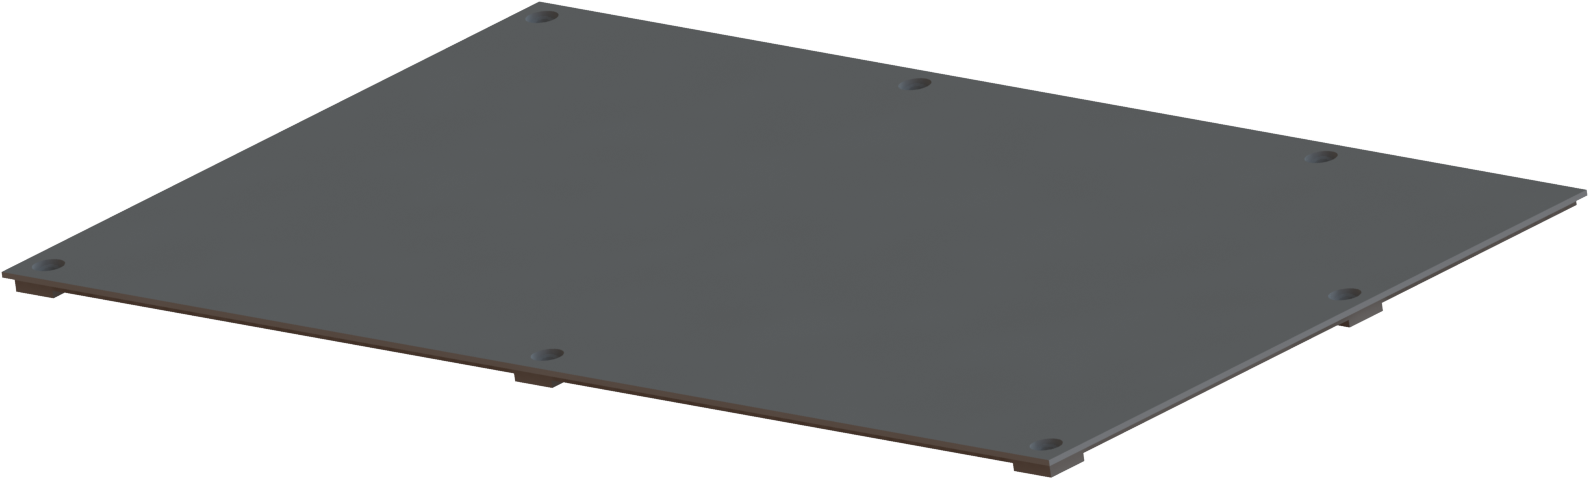
\includegraphics[scale=0.3]{Imagens/SW_Images/dalle_pad_capa_inferior.png}
            	\caption[Parte inferior do invólucro]{Parte inferior do invólucro}
            	\label{fig:bottom_dalle_pad}
            \end{figure}
            
            Também foi montada uma placa para os LED's centrais do produto e o botão que os controla. A parte superior do invólucro contém um encaixe para que esta peça permaneça firme, independente da pressão realizada sobre o botão. A figura ~\ref{fig:pcb_leds} apresenta o quão simples esta peça é:
            
            \begin{figure}[H]
                \centering
                \begin{subfigure}{.5\textwidth}
                  \centering
                  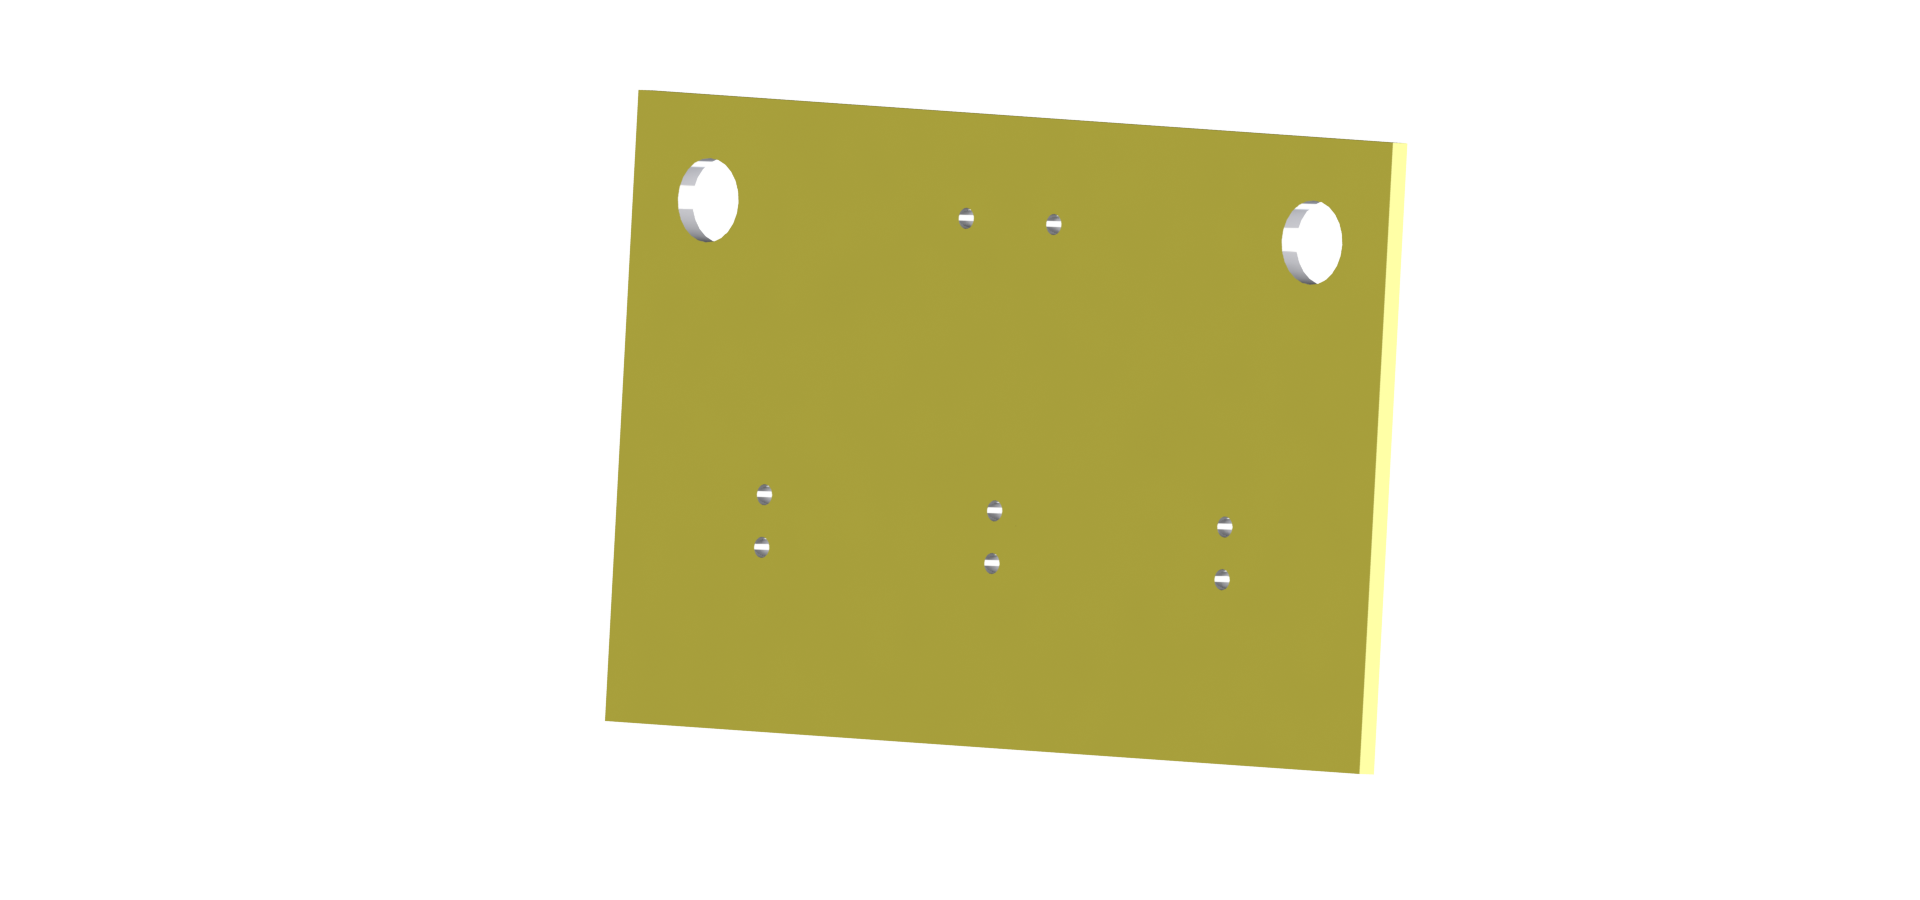
\includegraphics[scale=0.2]{Imagens/SW_Images/placa_universal_para_os_leds.png}
                  \caption{apenas a PCI}
                  \label{fig:just_leds_pcb}
                \end{subfigure}%
                \begin{subfigure}{.5\textwidth}
                  \centering
                  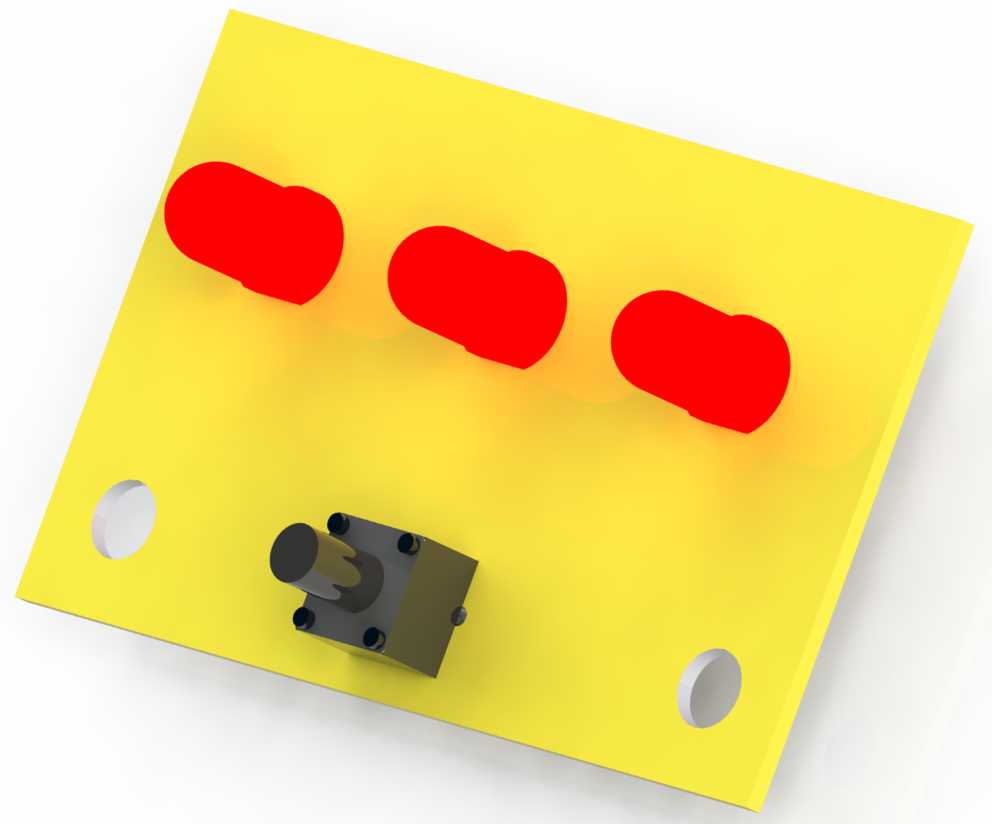
\includegraphics[scale=0.2]{Imagens/SW_Images/placa_universal_para_os_leds_montada.png}
                  \caption{PCI montada}
                  \label{fig:pcb_leds_full}
                \end{subfigure}
                \caption{PCI para os LED's centrais}
                \label{fig:pcb_leds}
            \end{figure}
        
        \subsection{Produto final}
        
            Com todos os componentes projetados e em mãos, pôde-se montar o produto final.
            
            
        